\section{Background and Motivation}
\label{SEC:background}


\subsection{Our Motivating Example}

% How SEA showed success using system calls

The initial impetus for this work came from our review
of earlier efforts by Moore et al. on the
the Simulating Environmental Anomalies (SEA) technique.
This effort centered on the key insight
that problematic
environmental properties,
known as anomalies, are visible in the
communications between the components that make up an application.
They found that,
once captured,
these anomalies
could be
used to create simulations
that test
an application as if
it had encountered the captured anomalies
in the real world.
In that work, SEA was used to test applications
by recording the system calls they made
during execution,
modifying the results of these calls such that a desired anomaly
was present,
and observing the application to see whether or not it
responded correctly to the anomaly.
Using this strategy, the authors were able to identify numerous bugs
in major applications~\cite{crashsim}.

Our takeaway
was that an application's activity
is a valuable resource that can be systematically mined
in order find to bugs
that may be missed by other techniques.
The work described in this paper
is based on our own key insight that that the best way to extract this
value
is to treat application activity
as a sequence of events
so that proven event processing techniques
may be employed in analyzing them.
Two realizations followed shortly after this
insight.
First was that, with the correct tools,
SEA's success in identifying environmental bugs using system calls
could be expanded
to encompass other activity types
like calls to library functions
and remote procedure calls.
Second was the understanding that existing tools,
while effective in their given areas,
are not up to the
task we had in mind.


%%% What are we really doing here.  WHY did we decided to make this language?
%%% That's really the question that needs to be answered.  I think that instead
%%% of making things up that we had the language and decided to apply it here
%%% we need to talk about how seeing the success of this work motivated us to
%%% try it at a larger scale.  We can avoid talk of "Augmenting" SEA or
%%% whatever though

\subsection{Expanding on Environmental Bugs}

Before we discuss the details of our bug-finding efforts it is necessary to
draw a boundary around the types of bugs we are targeting.
This work sets its sights on the bugs that occur when an some external
entity supplies unexpected or incorrect data to an
application resulting in its failure.
Such bugs may appear in simple situations such as a library function that
returns data in an unexpected format or in scenarios as complex
as a request to a remote
system returning bad data because of corruption on an intermediate network
node.
Both cases share the commonality that the symptoms of misbehavior are
visible in a recording of the applications activity.
These bugs, defined by Moore et al. as ``environmental bugs,''
often cause applications to fail after deployment
and occur with such frequency
that the ``works on my machine'' phenomenon is a well known
source of pain
and frequent topic of discussion
in software and project management
literature~\cite{notreal}.
The problem is so widespread
that FAKESTUDY concluded
that \$XXX are spent annually on efforts to
recall,
fix,
and re-deploy applications
because of all the bugs
that slipped past extensive testing efforts
during development.

The impact of these bugs continues to be reinforced by the regular
appearance of dangerous environmental bugs in major pieces of
software~\cite{devzeroroot}.  And it appears that no class of application
is safe with environmental bugs affecting operating systems~\cite{bad},
user applications~\cite{bad} and even web applications~\cite{bad} in the
last year alone!


\preston{Maybe I should include something here similar to the list from the
CrashSim paper that talks about different environmental bug sources in more
detail?}



\subsection{Why a New Programming Language?}
\begin{figure}
  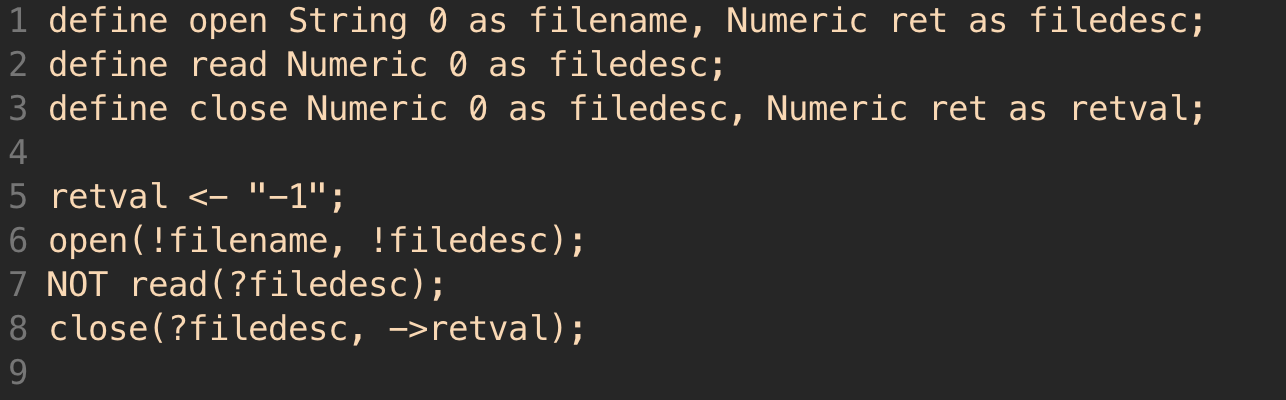
\includegraphics[scale=.50, frame]{images/cslanglisting}
  \caption{A listing of a cslang program.  This program finds situations
  where a program opens a file and closes it without reading from it.  In
  such instances, it modifies the return value close call to be -1,
  indicating failure.}
  \label{fig:cslanglisting}
\end{figure}

\begin{figure}
  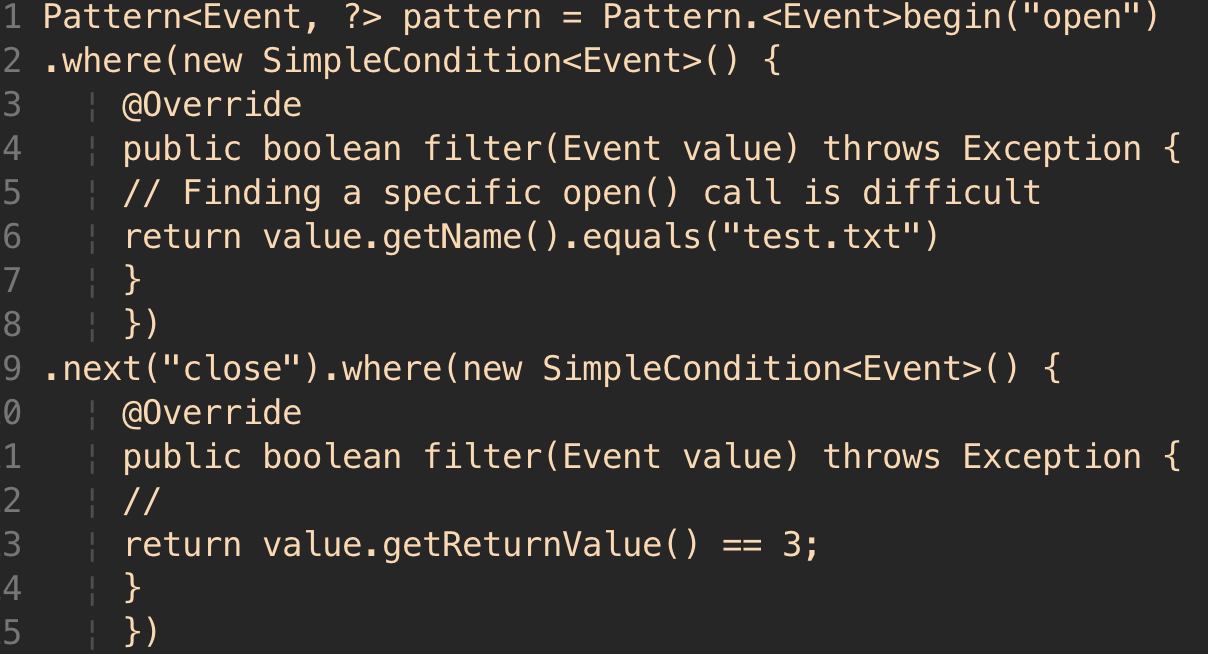
\includegraphics[scale=.50, frame]{images/flinklisting}
  \caption{A listing of an Apache Flink program that does the same thing as the
  cslang program... I need to figure out what comparison stuff to put in
  this caption.}
  \label{fig:flinklisting}
\end{figure}


The decision to create a new programming language was not one we
undertook lightly,
as such an effort takes
a significant amount of work
to define,
implement, document, and support.
In this section we discuss the features we needed for this work
and why existing systems fell short.

First, we needed a language that treated state as a first-class citizen.
That is, it must allow the internal contents of events like argument data,
pointer addresses, and return values to be easily captured, manipulated, and
reused in subsequent operations.
This is necessary because,
at a very high level,
the purpose of system calls,
function calls,
rpc calls,
or other similar activity
is to allow an application
to gather data from an external module like a library or the operating
system.
As a result, it is frequently useful to be able to store the data returned by
one such action, modify it, and use it in matching actions.
For example, one may store the file descriptor returned by a {\tt
socket()} system call and use it later to match other related
communication system calls.
We found that this sort of usage was common across many types of
application activity further reinforcing our desire for a language that was
closely tailored to our needs on this in this area.

% Need to support new event stream formats easily?


\preston{We need to make sure we have given a best effort at shortening and
optimizing code from other languages with which we are making comparisons}

Our second requirement appears to be largely aesthetic at first glance
but there is a
larger purpose -- ease of learning and ease of use.  CSlang offers
improvements over existing languages along two primary fronts.
First, many event processing languages are verbose.
Consider figure~\ref{fig:cslanglisting}  which shows a
CSLang program that matches sequences where an application opens and closes
a file without reading from it.  When such a sequence is found, it is
modified such that the {\tt close()} call returns -1, indicating failure.
The main work of this program is performed in just four lines of CSlang
code.  For comparison, figure~\ref{fig:flinklisting} contains a Java program that
implements an approximation of the same program that was implemented in
CSlang~\ref{fig:cslanglisting}.
This program is only an approximation because it does not modify the return
value of the close() call as the CSLang program does.  Further, it assumes
that other work has been done to modify Apache Flink to enable the
consumption of a sequence of system calls.
In spite of these shortcomings, comparing the two programs remains
enlightening.  The Flink program is harder to read because it contains a
great deal of boilerplate code
that cannot be avoided due to its dependence on a fully-featured
programming language.  Other work that explores how developers read and
understand (or mis-understand!) code has shown that such constructs obscure
a programs meaning, harming understanding and
maintainability~\ref{CITEATOMSWORK}.
In light of this, we believe the benefits of a
new programming language
focused on allowing its users to get a lot of work done
with a small amount of easily-readable code are evident.

The second front involves CSlang's programming paradigm.
While other event processing languages tend toward functional or
declarative programming,
CSlang programs more closely follow an imperative programming style.
We came to this decision because studies
have shown that developers are more likely to be familiar and comfortable
with such a paradigm~\cite{XXXX}.  We believe this will make it easier for
developers to learn the language, foster greater popularity, and it aligns
with the goals presented in our motivating example.

Our final requirement is, perhaps, the most important.
We want CSlang programs to be capable of more than simply matching
a pattern of events and indicating that it has occurred.
Our review of the work on the SEA technique has shown that the ability to
{\textit modify} is central to forcing an application into situations where
it may fail rather than only passively monitoring for it to perform
problematic sequences.  While the feature-rich nature of several related
languages and libraries means it is likely possible to modify and output
incoming events, it is by no means a straightforward
and ergonomic experience.
Constructing CSlang to support output as a primary feature allows us to
easily describe the types of transformations needed to expose bugs.


